%%%%%%%%%%%%%%%%%%%%%%%%%%%%
%LIEU
%%%%%%%%%%%%%%%%%%%%%%%%%%%%
\section{Le lieu}
%%%%%%%%%%%%%%%%%%%%%%%%%%%%
\subsection{Répartition des sources iconographiques (>100) par lieu}
\begin{lstlisting}[language=SQL, caption=Requête SQL pour nombre d'iconographies par lieu > 100]
SELECT place.id, place.id_richelieu,  
COUNT(r_iconography_place.id_iconography) AS total_icono_lieu 
FROM place 
JOIN r_iconography_place 
ON place.id = r_iconography_place.id_place 
JOIN iconography  
ON r_iconography_place.id_iconography = iconography.id 
GROUP BY place.id 
HAVING COUNT (*) > 100
ORDER BY total_icono_lieu desc; \end{lstlisting}

\begin{figure}[h!]
    \centering
    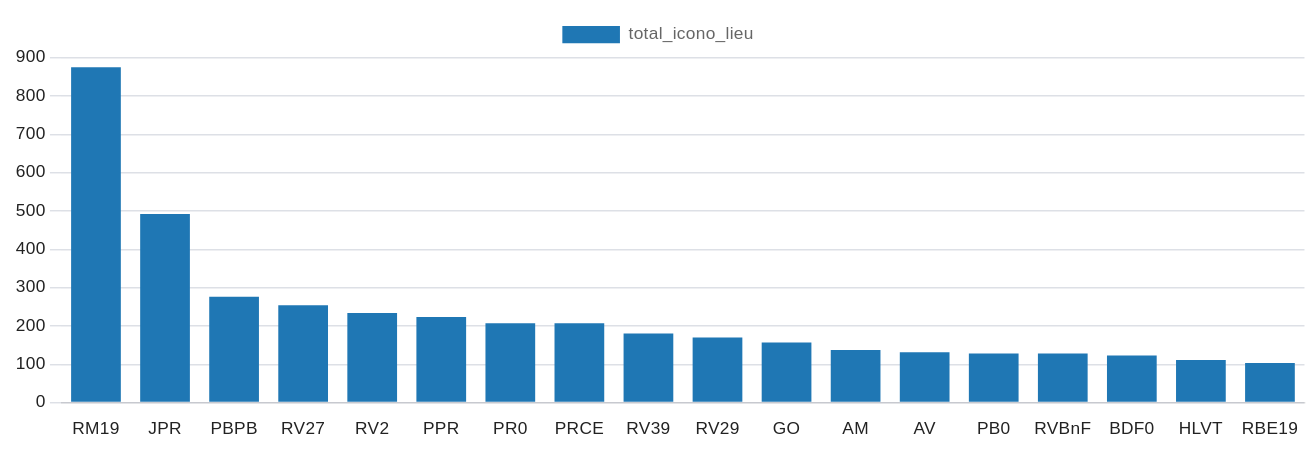
\includegraphics[width=1\linewidth]{images/graphiques/nb_icono_lieu_>100.png}
    \caption{Nombre d'iconographie par lieu (avec au moins 100 documents)}
    \label{fig:nb_icono_lieu>100}
\end{figure}    

\newpage
%%%%%%%%%%%%%%%%%%%%%%%%%%%%
\subsection{Répartition des sources cartographiques par lieu}
\begin{lstlisting}[language=SQL, caption=Requête SQL pour répartition des sources cartographiques par lieu]
SELECT place.id, place.id_richelieu,  
COUNT(r_cartography_place.id_cartography) AS total_carto_parcelle 
FROM place 
JOIN r_cartography_place 
ON place.id = r_cartography_place.id_place 
JOIN cartography  
ON r_cartography_place.id_cartography = cartography.id 
GROUP BY place.id 
ORDER BY total_carto_parcelle desc;\end{lstlisting}
\begin{figure}[h!]
    \centering
    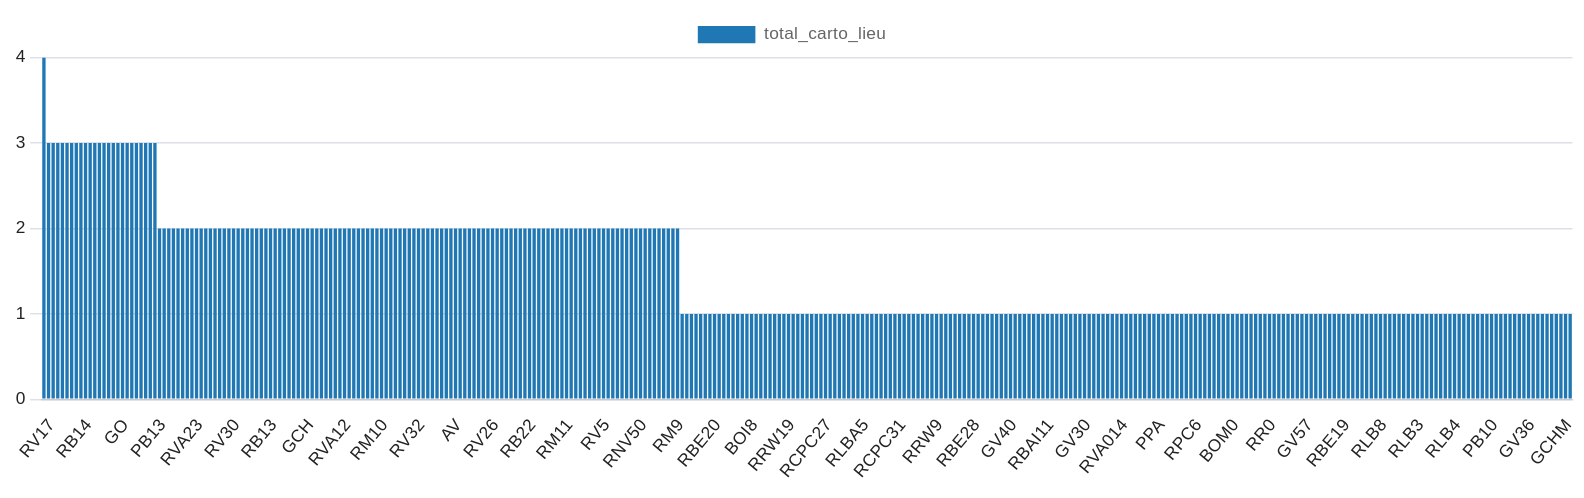
\includegraphics[width=1\linewidth]{images/graphiques/nb_carto_lieu_barChart.png}
    \caption{Nombre de sources cartographiques par lieu}
    \label{fig:nb_carto_lieu}
\end{figure}         

\begin{lstlisting}[language=SQL, caption=Reuquête SQL sur les lieux par nombre de documents cartographiques]
SELECT 
    lieu AS total_carto_lieu, 
    COUNT(id_richelieu) AS nombre_id_richelieu
FROM (
    SELECT place.id_richelieu, 
           COUNT(r_cartography_place.id_cartography) AS lieu 
    FROM place 
    JOIN r_cartography_place 
    ON place.id = r_cartography_place.id_place 
    JOIN cartography  
    ON r_cartography_place.id_cartography = cartography.id 
    GROUP BY place.id_richelieu 
) AS subquery
GROUP BY lieu
ORDER BY lieu;\end{lstlisting}

\begin{figure}[h!]
    \centering
    
\includegraphics[width=1\linewidth]{images/graphiques/repartition_lieux_nb_carto_lieu_pie.png}
    \caption{Répartition total des lieux en fonction du nombre de documents cartographiques par lieu.}
    \label{fig:repartition_carto_lieu}
\end{figure}

\begin{table}[h!]
    \centering
    \begin{tabular}{|l|r|}
        \toprule
        \textbf{Nb source carto} & \textbf{Nb lieux} \\
        \midrule
        1 & 193 \\
        2 & 113 \\
        3 & 24 \\
        4 & 1 \\
        \bottomrule
    \end{tabular}
    \label{tab:repartition_lieu_carto}
    \caption{Répartition totale du nombre de source cartographique par lieu.}
\end{table}

\newpage
%%%%%%%%%%%%%%%%%%%%%%%%%%%%
\subsection{Répartition toutes sources confondues par lieu}
\begin{lstlisting}[language=SQL, caption=Requête SQL pour répartition des sources par lieu]
SELECT subquery.id, subquery.id_richelieu, subquery.total_sources_lieu
FROM (
    SELECT p.id, p.id_richelieu,  
        COALESCE(carto.total_carto_lieu, 0) + COALESCE(icono.total_icono_lieu, 0) AS total_sources_lieu
    FROM place p
    LEFT JOIN (
        SELECT place.id, 
        COUNT(r_cartography_place.id_cartography) AS total_carto_lieu 
        FROM place 
        JOIN r_cartography_place 
        ON place.id = r_cartography_place.id_place 
        JOIN cartography  
    	ON r_cartography_place.id_cartography = cartography.id 
        GROUP BY place.id
    ) AS carto 
    ON p.id = carto.id
    LEFT JOIN (
        SELECT place.id, 
        COUNT(r_iconography_place.id_iconography) AS total_icono_lieu 
        FROM place 
        JOIN r_iconography_place 
        ON place.id = r_iconography_place.id_place 
        JOIN iconography  
        ON r_iconography_place.id_iconography = iconography.id 
        GROUP BY place.id
    ) AS icono 
    ON p.id = icono.id
) AS subquery
ORDER BY subquery.total_sources_lieu DESC;\end{lstlisting}

\begin{figure}[h!]
    \centering
    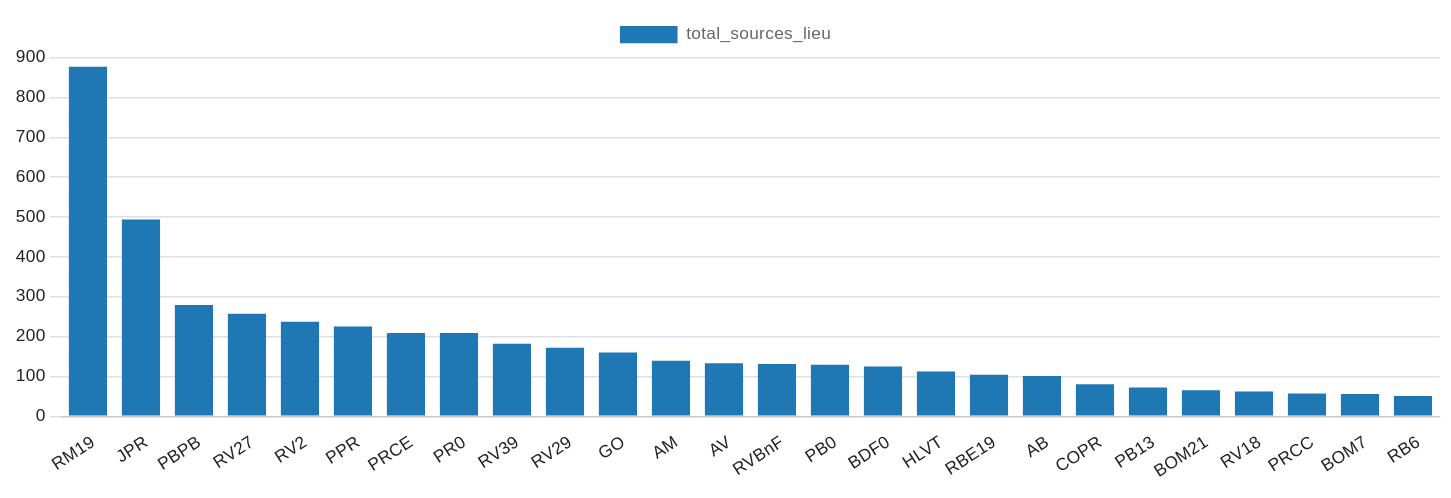
\includegraphics[width=1\linewidth]{images/graphiques/total_source_lieu.png}
    \caption{Répartition totale des sources par lieu}
    \label{fig:total_source_lieu}
\end{figure}
\newpage
%%%%%%%%%%%%%%%%%%%%%%%%%%%%
%CORPUS
%%%%%%%%%%%%%%%%%%%%%%%%%%%%
\section{Les corpus documentaires}
\subsection{La répartition des sources par institution}
\begin{lstlisting}[language=SQL, caption=Requête SQL pour nombre total de sources par institution]
SELECT 
    i.entry_name AS nom_institution,
    COALESCE(icono.nb_iconographie, 0) AS nb_iconographie,
    COALESCE(carto.nb_cartographie, 0) AS nb_cartographie,
    COALESCE(icono.nb_iconographie, 0) + COALESCE(carto.nb_cartographie, 0) AS total_resources
FROM institution AS i
LEFT JOIN (
    SELECT r.id_institution, COUNT(r.id_iconography) AS nb_iconographie
    FROM r_institution AS r 
    JOIN iconography AS ic 
        ON r.id_iconography = ic.id 
    GROUP BY r.id_institution
) AS icono 

ON i.id = icono.id_institution

LEFT JOIN (
    SELECT r.id_institution, COUNT(r.id_cartography) AS nb_cartographie 
    FROM r_institution AS r 
    JOIN cartography AS ic 
        ON r.id_cartography = ic.id 
    GROUP BY r.id_institution
) AS carto 

ON i.id = carto.id_institution
WHERE COALESCE(icono.nb_iconographie, 0) + COALESCE(carto.nb_cartographie, 0) > 50
ORDER BY total_resources DESC; \end{lstlisting}
\begin{figure}[h!]
    \centering
    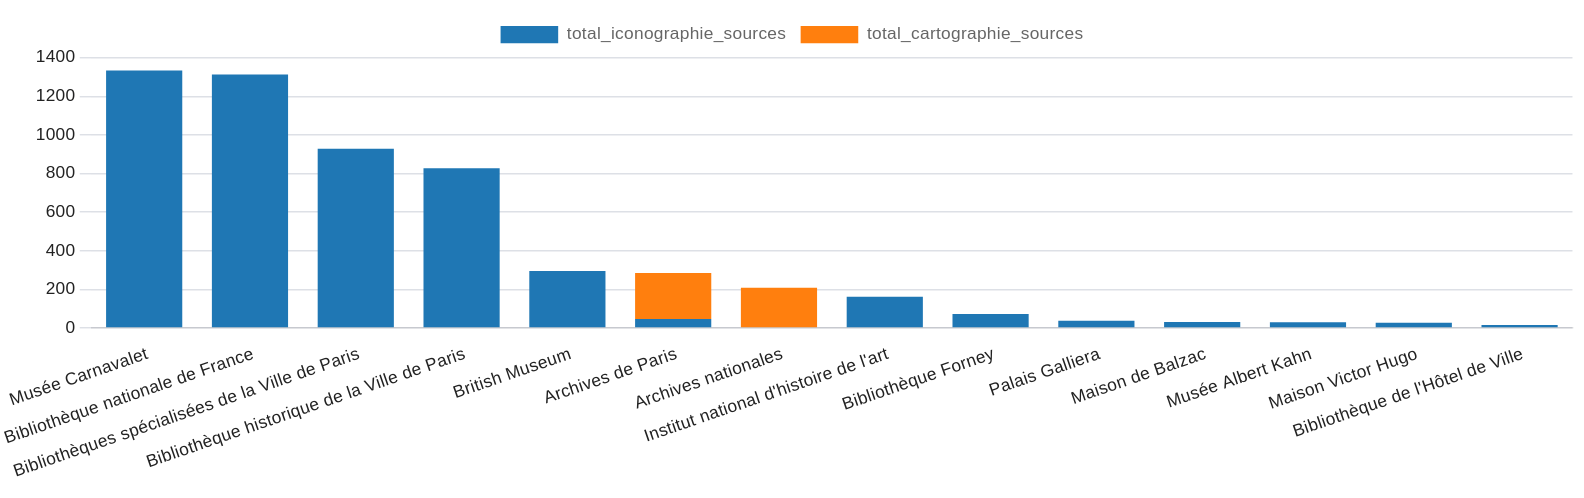
\includegraphics[width=1\linewidth]{images/graphiques/total_source_institution.png}
    \caption{Nombre total de sources par institution}
    \label{fig:total_sources_institution}
\end{figure}

% \begin{table}
% \begin{tabular}{|l|r|r|r|}
% \centering
% \textbf{Nom de l'institution} & \textbf{Nb iconographie} & \textbf{Nb cartographie} & \textbf{Total source} \\
% Paris Musées & 1438 & 22 & 1460 \\
% Musée Carnavalet & 1333 & 0 & 1333 \\
% Bibliothèque nationale de France & 1312 & 0 & 1312 \\
% Bibliothèques spécialisées de la Ville de Paris & 928 & 0 & 928 \\
% Bibliothèque historique de la Ville de Paris & 827 & 0 & 827 \\
% British Museum & 295 & 0 & 295 \\
% Archives de Paris & 46 & 239 & 285 \\
% Archives nationales & 0 & 208 & 208 \\
% Institut national d'histoire de l'art & 162 & 0 & 162 \\
% Bibliothèque Forney & 73 & 0 & 73 \\
% \end{tabular}
% \caption{Répartition totale des sources par institution}
% \label{tab:resources}
% \end{table}

\newpage
%%%%%%%%%%%%%%%%%%%%%%%%%%%%
\subsection{La répartition des iconographiques par medium}
\begin{lstlisting}[language=SQL, caption=Requête SQL pour nombre d'iconographies par technique]
SELECT 
    CASE 
    WHEN EXISTS (
        SELECT 1 
        FROM unnest(technique) AS t
        WHERE t ~* 'photographie'
        ) THEN 'photographie'
        WHEN EXISTS (
        SELECT 1 
        FROM unnest(technique) AS t
        WHERE t ~* 'gravure' OR t ~* 'estampe' OR t ~* 'lithographie'
        ) THEN 'estampe'
        WHEN EXISTS (
        SELECT 1 
        FROM unnest(technique) AS t
        WHERE t ~* 'dessin'
        ) THEN 'dessin'
        WHEN EXISTS (
        SELECT 1 
        FROM unnest(technique) AS t
        WHERE t ~* 'négatif'
        ) THEN 'négatif'
        WHEN EXISTS (
        SELECT 1 
        FROM unnest(technique) AS t
        WHERE t ~* 'plan'
        ) THEN 'plan'
        WHEN EXISTS (
        SELECT 1 
        FROM unnest(technique) AS t
        WHERE t ~* 'tableau' OR t ~* 'peinture'
        ) THEN 'peinture'
        ELSE array_to_string(technique, ', ')
        END AS type_regroupe,
    COUNT(*) AS nombre
    FROM iconography
GROUP BY type_regroupe
HAVING COUNT(*) > 10
ORDER BY nombre DESC; \end{lstlisting}

\begin{figure}[h!]
    \centering
    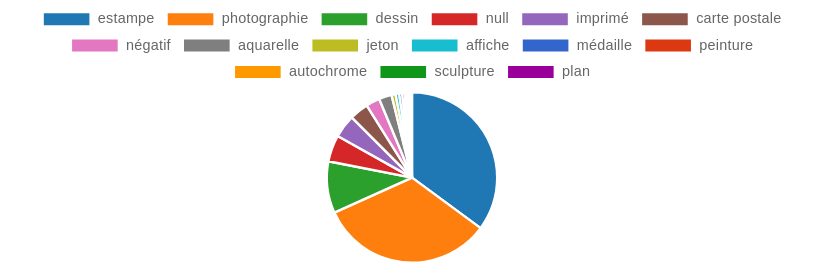
\includegraphics[width=1\linewidth]{images/graphiques/nb_icono_technique>10.png}
    \caption{Nombre d'iconographie par technique (en excluant celles de moins de 10 occurrences)}         \label{fig:nb_icono_technique}
\end{figure}

\begin{table}[h!]
    \centering
    \begin{tabular}{|l|r|}
        \toprule
        \textbf{Technique} & \textbf{Nombre} \\ \hline
        estampe        & 1436 \\ 
        photographie   & 1357 \\ 
        dessin         & 401  \\ 
        \texttt{NULL}  & 206  \\ 
        imprimé        & 179  \\ 
        carte postale  & 147  \\ 
        négatif        & 108  \\
        aquarelle      & 99   \\
        jeton          & 31   \\
        affiche        & 28   \\
        médaille       & 23   \\
        peinture       & 21   \\
        autochrome     & 19   \\
        sculpture      & 18   \\
        plan           & 18   \\ 
        \midrule
        \textbf{Total} & 4091 \\
        \bottomrule
    \end{tabular}
    \caption{Répartition des types d'iconographies}
    \label{tab:repartition_iconographies}
\end{table}

\newpage
%%%%%%%%%%%%%%%%%%%%%%%%%%%%
%TEMPS
%%%%%%%%%%%%%%%%%%%%%%%%%%%%
\section{Le temps}
\subsection{La répartition temporelle des sources : par intervalle de 50 ans}
\begin{lstlisting}[language=SQL, caption=Requête SQL pour nombre de sources par date (50 ans)]
SELECT
    periode,
    SUM(nombre_documents) AS nombre_documents,
    SUM(nombre_iconographies) AS nombre_iconographies,
    SUM(nombre_cartographies) AS nombre_cartographies
FROM (
    SELECT 
        CASE 
            WHEN iconography.date && int4range(1200, 1750) THEN 'avant1750'
            WHEN iconography.date && int4range(1750, 1800) THEN '1750-1800'
            WHEN iconography.date && int4range(1800, 1850) THEN '1800-1850'
            WHEN iconography.date && int4range(1850, 1900) THEN '1850-1900'
            WHEN iconography.date && int4range(1900, 1950) THEN '1900-1950'
            WHEN iconography.date && int4range(1950, 2100) THEN 'après1950'
        END AS periode,
        COUNT(*) AS nombre_documents,
        COUNT(*) AS nombre_iconographies,
        0 AS nombre_cartographies
    FROM 
        iconography
    GROUP BY 
        periode

    UNION ALL

    SELECT 
        CASE 
            WHEN cartography.date && int4range(1200, 1750) THEN 'avant1750'
            WHEN cartography.date && int4range(1750, 1800) THEN '1750-1800'
            WHEN cartography.date && int4range(1800, 1850) THEN '1800-1850'
            WHEN cartography.date && int4range(1850, 1900) THEN '1850-1900'
            WHEN cartography.date && int4range(1900, 1950) THEN '1900-1950'
            WHEN cartography.date && int4range(1950, 2100) THEN 'après1950'
        END AS periode,
        COUNT(*) AS nombre_documents,
        0 AS nombre_iconographies,
        COUNT(*) AS nombre_cartographies
    FROM 
        cartography
    GROUP BY 
        periode
) AS combined_results
GROUP BY 
    periode
ORDER BY 
    CASE 
        WHEN periode = 'avant 1750' THEN 1
        WHEN periode = '1750-1800' THEN 2
        WHEN periode = '1800-1850' THEN 3
        WHEN periode = '1850-1900' THEN 4
        WHEN periode = '1900-1950' THEN 5
        WHEN periode = 'après 1950' THEN 6
    END; \end{lstlisting}
    
\begin{figure}[h!]
    \centering
    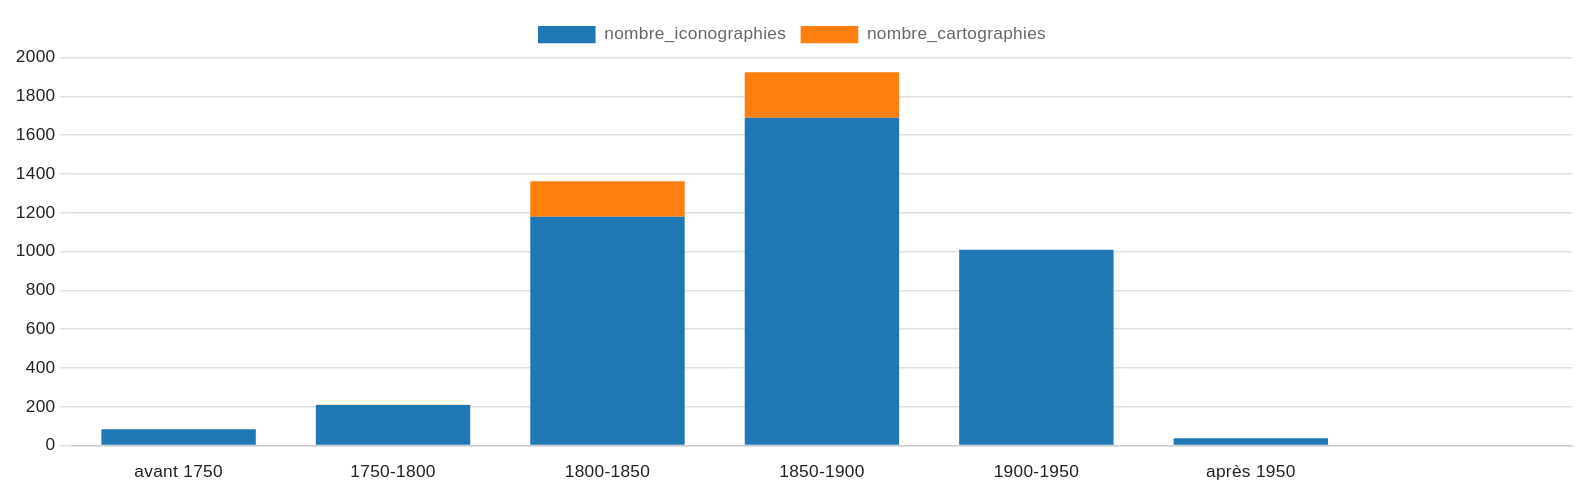
\includegraphics[width=0.75\linewidth]{images/graphiques/total_source_date_50.png}
    \caption{Nombre total de sources par date (intervalle de 50 ans)}
    \label{fig:total_sources_date50}
\end{figure}

\newpage
%%%%%%%%%%%%%%%%%%%%%%%%%%%%
\subsection{La répartition temporelle des sources : par intervalle de 10 ans}
\begin{lstlisting}[language=SQL, caption=Requête SQL pour nombre de sources par date (10 ans)]
SELECT COALESCE(c.periode, i.periode) AS periode, COALESCE(nb_carto_periode_10ans, 0) AS nb_carto_periode_10ans, COALESCE(nb_icono_periode_10ans, 0) AS nb_icono_periode_10ans
FROM 
    (SELECT CASE 
        WHEN cartography.date && int4range(1200, 1750) THEN '> 1750' 
        WHEN cartography.date && int4range(1750, 1760) THEN '1750-1760' 
        WHEN cartography.date && int4range(1760, 1770) THEN '1760-1770' 
        WHEN cartography.date && int4range(1770, 1780) THEN '1770-1780' 
        WHEN cartography.date && int4range(1780, 1790) THEN '1780-1790' 
        WHEN cartography.date && int4range(1790, 1800) THEN '1790-1800' 
        WHEN cartography.date && int4range(1800, 1810) THEN '1800-1810' 
        WHEN cartography.date && int4range(1810, 1820) THEN '1810-1820' 
        WHEN cartography.date && int4range(1820, 1830) THEN '1820-1830' 
        WHEN cartography.date && int4range(1830, 1840) THEN '1830-1840' 
        WHEN cartography.date && int4range(1840, 1850) THEN '1840-1850' 
        WHEN cartography.date && int4range(1850, 1860) THEN '1850-1860' 
        WHEN cartography.date && int4range(1860, 1870) THEN '1860-1870' 
        WHEN cartography.date && int4range(1870, 1880) THEN '1870-1880' 
        WHEN cartography.date && int4range(1880, 1890) THEN '1880-1890' 
        WHEN cartography.date && int4range(1890, 1900) THEN '1890-1900' 
        WHEN cartography.date && int4range(1900, 1910) THEN '1900-1910' 
        WHEN cartography.date && int4range(1920, 1930) THEN '1920-1930' 
        WHEN cartography.date && int4range(1930, 1940) THEN '1930-1940' 
        WHEN cartography.date && int4range(1940, 1950) THEN '1940-1950' 
        WHEN cartography.date && int4range(1950, 2100) THEN '< 1950' 
        END AS periode, 
        COUNT(*) AS nb_carto_periode_10ans
    FROM cartography 
    GROUP BY periode 
    ORDER BY periode) c
FULL OUTER JOIN 
    (SELECT CASE 
        WHEN iconography.date && int4range(1200, 1750) THEN '> 1750' 
        WHEN iconography.date && int4range(1750, 1760) THEN '1750-1760' 
        WHEN iconography.date && int4range(1760, 1770) THEN '1760-1770' 
        WHEN iconography.date && int4range(1770, 1780) THEN '1770-1780' 
        WHEN iconography.date && int4range(1780, 1790) THEN '1780-1790' 
        WHEN iconography.date && int4range(1790, 1800) THEN '1790-1800' 
        WHEN iconography.date && int4range(1800, 1810) THEN '1800-1810' 
        WHEN iconography.date && int4range(1810, 1820) THEN '1810-1820' 
        WHEN iconography.date && int4range(1820, 1830) THEN '1820-1830' 
        WHEN iconography.date && int4range(1830, 1840) THEN '1830-1840' 
        WHEN iconography.date && int4range(1840, 1850) THEN '1840-1850' 
        WHEN iconography.date && int4range(1850, 1860) THEN '1850-1860' 
        WHEN iconography.date && int4range(1860, 1870) THEN '1860-1870' 
        WHEN iconography.date && int4range(1870, 1880) THEN '1870-1880' 
        WHEN iconography.date && int4range(1880, 1890) THEN '1880-1890' 
        WHEN iconography.date && int4range(1890, 1900) THEN '1890-1900' 
        WHEN iconography.date && int4range(1900, 1910) THEN '1900-1910' 
        WHEN iconography.date && int4range(1920, 1930) THEN '1920-1930' 
        WHEN iconography.date && int4range(1930, 1940) THEN '1930-1940' 
        WHEN iconography.date && int4range(1940, 1950) THEN '1940-1950' 
        WHEN iconography.date && int4range(1950, 2100) THEN '< 1950' 
        END AS periode, 
        COUNT(*) AS nb_icono_periode_10ans
    FROM iconography 
    GROUP BY periode 
    ORDER BY periode) i
ON c.periode = i.periode
ORDER BY periode; \end{lstlisting}

\begin{figure}[h!]
    \centering
    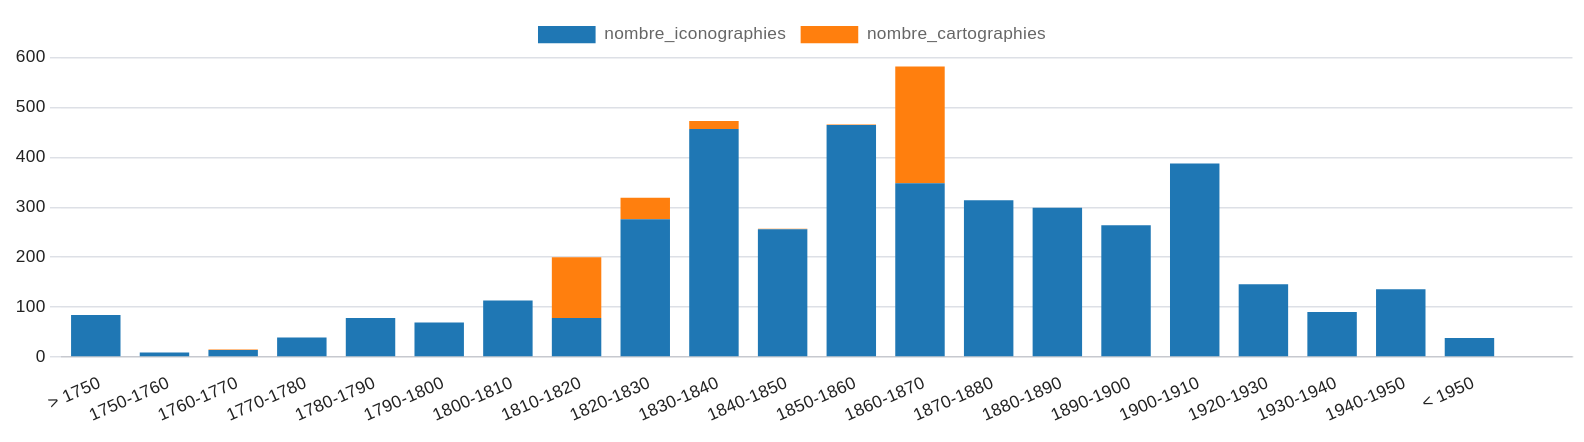
\includegraphics[width=1\linewidth]{images/graphiques/total_source_date_10.png}
    \caption{Total des sources par date (intervalle de 10 ans)}
    \label{fig:total_sources_date10}
\end{figure}